\documentclass[10pt,fleqn]{article}

\usepackage[english]{babel}
\usepackage[utf8x]{inputenc}
\usepackage{enumerate}
\usepackage{amsmath}
\usepackage{amssymb}
\usepackage{amsfonts} 
\usepackage{mathtools}
\usepackage{graphicx}
\usepackage{bm}
\usepackage[usenames,dvipsnames]{color}
\usepackage{todonotes}
\usepackage{dsfont}
\usepackage{hyperref}
\hypersetup{
    colorlinks,
    citecolor=black,
    filecolor=black,
    linkcolor=black,
    urlcolor=black
}
\usepackage{algorithm}
\usepackage{algorithmic}
\usepackage{appendix}
\usepackage{subcaption}
\usepackage{fancyvrb}
\usepackage{subfigure}
\usepackage{graphicx,xcolor}
\usepackage{pifont,mdframed}
\usepackage{tikz}
\usepackage{bm}
\usetikzlibrary{fit,positioning}


%
% Macros
%
\newcommand \cashort[1] { {\todo[color=yello]{#1 -- Cedric}} }
\newcommand \calong[1]  { { \todo[inline,color=yellow]{#1 -- Cedric} } }
\newcommand \gbshort[1] { {\todo[color=cyan!40]{#1 -- Guillaume}} }
\newcommand \gblong[1]  { { \todo[inline, color=cyan!40]{#1 -- Guillaume} } }
\newcommand \mgshort[1] { {\todo{#1 -- Mark}} }
\newcommand \mglong[1]  { { \todo[inline]{#1 -- Mark} } }
\newcommand \bfshort[1] { {\todo[color=green!40]{#1 -- Bryan}} }
\newcommand \bflong[1]  { { \todo[inline,color=green!40]{#1 -- Bryan} } }


% Adds a plus const to the end of a math expression
\def \pcst{+\text{const}}

% A fancy version for capital R
\def \Rcal{\mathcal{R}}

% A fancy version for r
\def \rcal{\mathbf{r}}

% Loss function / log likelihood as appropriate
\def \L{\mathcal{L}}

% KL divergence [Math Mode]
\newcommand{\kl}[2] {
	\text{KL}\left[#1||#2\right]
}

\newcommand \vecf[1] {
    \text{vec}\left(#1\right)
}

\newcommand \ent[1] {
    \text{H} \left[ #1 \right]
}

\newcommand \mut[2] {
    \text{I} \left[ #1 ; #2 \right]
}

\newcommand \dvi[2] {
    \text{D}_\text{VI} \left[ #1; #2 \right]
}

% Starts an expected value expresses [Math Mode]
\newcommand{\starte}[1] {%
	\mathbb{E}_{#1}\left[
}

% Ends an expected value expression [Math Mode]
\def \ende{\right]}

% Starts an varianc expresses [Math Mode]
\newcommand{\startv}[1] {%
	\mathbb{V}\text{ar}_{#1}\left[
}

% Ends an variance expression [Math Mode]
\def \endv{\right]}

%\newcommand \ex[2] {
%    \bigl\langle #1 \bigr\rangle_{#2}
%}
\newcommand \ex[2] {
    \mathbb{E}_{ { #2 } }\left[ #1 \right]
}
\newcommand \var[2] {
    \mathbb{V}ar_{ { #2 } }\left[ #1 \right]
}

\newcommand \halve[1] {
	\frac{#1}{2}
}

\newcommand \half {
    \halve{1}
}

\newcommand \tr { \text{tr} } 

\newcommand \T { ^\top } 

\newcommand \fixme[1] {
    {\color{red} FIXME: #1}
}

\newcommand \vv[1] { \bm #1 }

\newcommand{\mbeq}{\overset{!}{=}}

\newcommand \diag[1] { \text{diag} \left( {#1} \right) }
\newcommand \diagonal[1] { \text{diagonal} \left( {#1} \right) }

\newcommand \Ed {{ \vv{\xi}_d}}
\newcommand \Edj {{\xi_{dj}}}
\newcommand \Edk {{\xi_{dk}}}
\newcommand \AEdj {{\Lambda(\xi_{dj})}}
\newcommand \AEdk {{\Lambda(\xi_{dk})}}
\newcommand \AEd  {{ \bm{\Lambda}(\bm{\xi}_d) }}

\newcommand \Axi { { \Lambda_{\xi} } }
\newcommand \bxi { { \vv{b}_{\xi} } }
\newcommand \cxi { { c_{\xi} } }


\newcommand \wdoc      { { \vv{w}_d } }
\newcommand \wdt[0]  { { w_{dt} } }
\newcommand \wdn[0]  { { \vv{w}_{dn} } }
\newcommand \wdnt[0]  { { w_{dnt} } }
\newcommand \wdd[0]   { { \vv w_{d} } }
\newcommand \zd[0]   { { \vv z_{d} } }
\newcommand \zdn[0]  { { \vv{z}_{dn} } }
\newcommand \zdnk[0] { { z_{dnk} } }
\newcommand \zdk[0]  { { z_{dk} } }
\newcommand \thd[0]  { { \vv \theta_d } }
\newcommand \thdk[0] { { \theta_{dk} } }
\newcommand \thdj[0] { { \theta_{dj} } }
\newcommand \epow[1] { { e^{#1} } }
\newcommand \pkt     { { \phi_{kt}  } }
\newcommand \pk      { { \vv \phi_k } }
\newcommand \lmd     { { \vv \lambda_d } }
\newcommand \lmdk    { { \lambda_{dk} } }
\newcommand \xd      { { \vv x_d } }
\newcommand \atxd     { A ^\top \bm x_d}
\newcommand \axd     { A\bm x_d}
\newcommand \tsq      { { \tau^2 } }
\newcommand \ssq      { { \sigma^2 } }
\newcommand \tmsq     { { \tau^{-2} } }
\newcommand \asq      { { \alpha^2 } }
\newcommand \amsq     { { \alpha^{-2} } }
\newcommand \sgsq     { { \sigma^2 } }
\newcommand \xvec     { { \vv{x} } }
\newcommand \omk      { { \bm \omega _k } }
\newcommand \omkt     { { \omega_{kt} } }
\newcommand \oma     { { \Omega_A } }
\newcommand \gdn      { { \vv{\gamma}_{dn} } }
\newcommand \gdnk     { { \gamma_{dnk} } }
\newcommand \gdk      { { \gamma_{dk} } }
\newcommand \isigt   { { \Sigma^{-1}_{\bm \theta} } }




\newcommand \halfSig { \frac{1}{2\sigma^2} }

\newcommand \nor[2]   { \mathcal{N} \left( {#1}, {#2} \right) }
\newcommand \nord[3]   { \mathcal{N}_{#1} \left( {#2}, {#3} \right) }
\newcommand \mnor[3]  { \mathcal{N} \left(#1, #2, #3\right) }
\newcommand \norp[3]  { \mathcal{N} \left(#1; #2, #3\right) }
\newcommand \mnorp[4] { \mathcal{N} \left(#1; #2, #3, #4\right) }
\newcommand \mul[1]   { \mathcal{M} \left( {#1} \right) }
\newcommand \muln[2]  { \mathcal{M} \left( {#1},{#2} \right) }
\newcommand \dir[1]   { \mathcal{D} \left( {#1} \right) }
\newcommand \pois[1]  { \mathcal{P} \left( {#1} \right) }
\newcommand \gp[2]    { \mathcal{GP} \left( {#1}, #2 \right) }
\newcommand \dir[1]   { \mathcal{D} \left( {#1} \right) }
\newcommand \gam[2]   { \mathcal{G} \left( {#1}, {#2} \right) }
\newcommand \beta[1]  { \mathcal{B}eta \left( {#1}, {#2} \right) }

\newcommand \lne[1]  { { \ln \left( 1 + e^{ #1 } \right) } }
\newcommand \Tr[1]   { \tr \left(  {#1}  \right) }

\newcommand \roud  { \vv{\rho}_{d}  }
\newcommand \rodk { \rho_{dk} }

\newcommand \exA[1]  { \ex{#1}{q(A)} }
\newcommand \exV[1]  { \ex{#1}{q(V)} }
\newcommand \exT[1]  { \ex{#1}{q(\Theta)} }
\newcommand \extd[1] { \ex{#1}{q(\thd)} }
\newcommand \exTV[1] { \ex{#1}{q(\Theta)q(V)} }

\newcommand \Real[0]  { { \mathbb{R} } }
\newcommand \VReal[1] { { \mathbb{R}^{#1} } }
\newcommand \MReal[2] { { \mathbb{R}^{#1 \times #2} } }
\newcommand \Nat[0]  { { \mathbb{N} } }
\newcommand \VNat[1] { { \mathbb{N}^{#1} } }
\newcommand \MNat[2] { { \mathbb{N}^{#1 \times #2} } }

\newcommand \inv[1] { {#1}^{-1} }
\newcommand \invb[1] { \inv{\left( #1 \right)} }

\newcommand \cn { \textsuperscript{\texttt{[{\color{blue}Citation Needed}]}} }

\newcommand \const { { \text{c} } }

\providecommand \floor [1] { \left \lfloor #1 \right \rfloor }
\providecommand \ceil [1] { \left \lceil #1 \right \rceil }


\newcommand \vt[2] { { #1^{(#2)} } }

\newcommand \hashtag[1] { { \ttfamily \##1 } }

\newcommand \mvy  { \vv{m}_{\vv{y}} }
\newcommand \sigvy { { S_Y } }

\newcommand \mmy  { M_Y      }
\newcommand \md   { \vv{m}_d }
\newcommand \phin { \vv{\phi}_n }
\newcommand \isigma { { \inv{\Sigma} } }

\newcommand \sigv     { { \Sigma_V } }
\newcommand \isigv     { { \Sigma^{-1}_V } }

\newcommand \sigy { { \Sigma_Y } }
\newcommand \isigy { { \Sigma_{-1}_Y } }


\newcommand \omy  { { \Omega_Y } }
\newcommand \iomy { { \inv{\Omega_Y} } }

\newcommand \siga     { { \Sigma_A } }
\newcommand \isiga     { { \Sigma^{-1}_A } }
\newcommand \diagv { { \diag{\nu_1,\ldots,\nu_P} } }

\newcommand \ma { \vv{m}_a }
\newcommand \my { \vv{m}_y }

\newcommand \VoU { V \otimes U }

\newcommand \one { \mathbb{1} }
%\newcommand \one  {{  \mathds{1} }}

\newcommand \lse { \text{lse} }
%\newcommand \lse[0] { \mathrm{lse} }

% Conditional independence 
\def\ci{\perp\!\!\!\perp} % from Wikipedia



% ------ For the eval section

% Multinomial PDF [Math Mode]
% params: 1 - the variable
%         2 - the value
%         3 - the state indicator (e.g. k for a distro with K values)
%         4 - any additional subscript
\newcommand{\mpdf}[4] {
	\prod_{#3} {#1}_{{#4} {#3}} ^ {#2}
}

% Dirichlet PDF [Math Mode]
% params: 1 - the variable
%         2 - the hyper-parameter
%         3 - the state indicator (e.g. k for a distro with K values)
%         4 - any additional subscript
\newcommand{\dpdf}[4] {
	\frac{1}{B({#2})} \prod_{#3} {#1}_{{#4} {#3}} ^ {({#2}_{#3} - 1)}
}

% To simplify the sampling equations, this is indicates
% that the given value has had datapoint "m" stripped out
%
\newcommand{\lm}[1] {
	#1^{\setminus m}
}

\newcommand \model[0] {
    \mathcal{M}
}

\newcommand \perplexity[1] {
    \mathcal{P} \left( { #1 } \right)
}

\newcommand \WTrain {
    \mathcal{W}^{(t)}
}

\newcommand \WQuery {
    \mathcal{W}^{(q)}
}

\newcommand \oneover[1] {
    \frac{1}{ {#1} }
}

\newcommand \samp[1] {
    { #1 }^{(s)}
}

\newcommand \etd[0] {
    \vv{\eta}_d
}

\begin{document}




\newcommand \xdat { { \mathcal{X} } }
\newcommand \xdoc { { \vv{x}_d } }
\newcommand \xdn { { \vv{x}_{dn} } }

\chapter{Non-Conjugate Bayesian Inference}
\label{sec:nonconj}
In this chapter we investigate several approximations to the log-sum-exp function which arises when working with the logit. We qualitatively and quantitatively evaluate several approximation techniques on two classes of model: logistic regression and the correlated topic-model (CTM).

In particular while Taylor approximations have been recommended for inference with the \cite{Wang2013} we investigate other families of approximations, and qualitiatively show that one, the Bohning bound\cite{Bohning1988} offers faster and more accurate convergence. 
\section{The Logit}
In the previous chapter we considered only those cases where the posterior and prior are conjugate, and so tractable closed-form updates can be easily derived. However there are many classes of model where conjugacy is not available. For example, in logistic regression one introduces an \emph{activation function} $f(y) : \mathbb{R} \rightarrow [0, 1]$ which maps the real number line onto the interval $[0,1]$.
\begin{align*}
p(t_d = 1) = & f(y_d) & d_n  & \sim \mathcal{B} \left( \vv{w}\T\vv{x}_d\right) & \vv{w} & \sim \nor{0}{\alpha^2 I} \\
\end{align*}
where $\mathcal{B}(\cdot)$ is the Bernoulli distribution.

We consider inference for two cases of two sigmoidal activation functions for which f(0) = 0.5: the probit $\Phi(a)$ and the logit $\sigma(a)$.

\subsection{Inference with the Logit}
The logit is motivated as a log-odds ratio. Let $y_d = \vv{w}\T\vv{x}_d$. Then:

\begin{alignat}{3}
\ln \frac{p(t_d = 1)}{p(t_d = 0)}  & = y_d  &
%\implies & \frac{p(t_n = 1)}{p(t_n = 0)}      & = e^{y_n} \\
\implies & \frac{p(t_d = 1)}{1 - p(t_d = 1)}  & = & e^{y_d} \\
& & \implies &  p(t_d = 1)                    & = & \frac{e^{y_d}}{1 + e^{y_d}} = \frac{1}{1+e^{-y_d}}
\end{alignat}

This leads to an easy interpretation of the weights in logistic regression: each individual weight $w_f$ indicates by how much the log-odds of the positive class are increased.

% FIXME comment again
The following identities are useful when working with the logit:
\begin{align}
\sigma(y)' & = \sigma(y)(1 - \sigma(y)) \label{eqn:sigma-identity} &
2 \sigma(y) & = 1 - \tanh (\frac{y}{2}) \\
1 - \sigma(y) & = \frac{e^{-y}}{1 + e^{-y}} &
\sigma(-y) & = -\sigma(y)
\end{align}


\subsection*{Maximum Likelihood Estimation}
With a Bernoulli distribution on $t_d$ the log-likelihood has the form

\begin{equation}
\begin{aligned}
\ln p(\vv{y}; X, \vv{w}) & = \sum_d t_d \ln \sigma(y_d) + (1 - t_d) \ln (1 - \sigma(y_d)) \\
& \text{where } y_d = \vv{w}\T\vv{x}_d
\end{aligned}
\end{equation}

Making use of the fact that the derivative $\sigma(y)' = \sigma(y)(1 - \sigma(y))$ and the chain-rule one obtains the following equations for the gradient $\vv{g}_w$ and Hessian $H_w$ of the log-likelihood with respect to $\vv{w}$.

\begin{align}
\vv{g}_w = & X\T (\vv{y} - \vv{t}) \label{eqn:logit-gradient}\\
H_w      = & X\T R X & R = & \diag{y_d (1 - y_d)} \label{eqn:logit-hessian}
\end{align}

from which the following Newton-Raphson update is derived
\begin{align}
\vv{w}^{(\text{new})} \leftarrow \vv{w}^{(old)} - H_w^{-1} \vv{g}_w
\end{align}

With some re-arrangement of \eqref{eqn:logit-gradient} and \eqref{eqn:logit-hessian} this can be re-written in the form of a weighted least-squares problem:

\begin{align}
\vv{w}^{(\text{new})} & = \left(X\T R X \right)^{-1} X\T R \vv{z} & \vv{z} = X \vv{w}^{(old)}-R^{-1}(\vv{y} - \vv{t})
\end{align}


\subsection*{MAP Estimation using Global Approximations}
\newcommand \wmap[0] { \vv{w}_{\text{\tiny \sc MAP}} }

Consider a zero-mean Gaussian prior on the weight
\begin{align}\vv{w} \sim & \nor{\vv{0}}{\Lambda} &
t_d | y_d \sim & \mathcal{B}\left( \sigma(y_d) \right) & 
y_d = \vv{w}\T\vv{x}_d  \label{eqn:bayes-logit-model}
\end{align}

This prior is not conjugate to the Bernoulli likelihood, so the posterior distribution on $\vv{w}$ cannot be derived analytically and is instead approximated by a Taylor approximation of the posterior. As described in \cite{Wang2013} the approximation can be taken about an arbitrary point, the true mean, or the mode; known as the log-concave bound, the delta method and the Laplace approximation respectively. We call these global approximations as we are using a \emph{single} approximation over a posterior distribution derived from the \emph{entire} dataset.

With reference to the Laplace approximation, the gradient at the mode is by definition zero, so the approximation is defined in terms of a quadratic function of the weights. Thus the Laplace approximation corresponds to the following Gaussian distribution:

\begin{equation}
p(\vv{w}|X,\vv{t}) \approx q(\vv{w}) = \nor{\wmap}{-\inv{H_w}}
\end{equation}

Following the central limit theorem, we would expect the Laplace approximation to better approximate the posterior as the number of datapoints increases. The MAP estimate of the weights $\vv{w}_{MAP}$ is found, as in the MLE case, by some iterative method such as Newton-Raphson. The the Hessian is defined as:

\begin{align}
H_w   & = \inv{\Lambda} + X\T R X & R = \diag{y_n(1 - y_n)} 
\end{align}

Having obtained a posterior distribution over the weights, it remains to obtain a valid predictive distribution for a new datapoint $\vv{x}_*$

\begin{align}
p(t_* = 1| \vv{x}_*, X, \vv{t}) & = \int p(t_*|\vv{w}, \vv{x}_*)p(\vv{w}|X,\vv{t}) d\vv{w} \label{eqn:log-reg-predict} \\
 & \approx \int \sigma(\vv{w}\T\vv{x}_*)q(\vv{w}) d\vv{w} \label{eqn:log-reg-predict-approx-q}
\end{align}

A number of approaches are available. The simplest approach is to assume the posterior is sharply peaked around the mean, and simply plug the posterior mean directly into the sigmoid so $p(t|\vv{x}_*, X, \vv{t}) \approx \sigma(\vv{w}_{\text{MAP}}^\top \vv{x}_*)$

A second approach is to use Monte-Carlo sampling to approximate the integral \eqref{eqn:log-reg-predict} using $q(\vv{w})$ as a proposal distribution.

A third method is the probit approximation\cite{Barber1998} to approximate the integral \eqref{eqn:log-reg-predict-approx-q}. By requiring both functions to have the same slope at the origin we can derive the approximation $\sigma(a) \approx \Phi(\lambda a)$ where $\lambda = \sqrt{\frac{\pi}{8}}$. As the convolution of the probit with a Gaussian is also a probit function\footnote{$\int \Phi(\lambda a)\norp{a}{\mu}{\sigma^2} \text{d}a = \Phi\left(\mu / (\lambda^{-2} + \sigma^2)^{\half} \right)$} we arrive at the following predictive distribution:


\begin{align}
p(t_* = 1 | \vv{x}_*, X, \vv{t}) = \sigma\left( \kappa(\sigma_y^2) \mu_y \right)
\end{align}
where
\begin{align}
\mu_y       & = \wmap\T\vv{x}_* &
\sigma_y    & = -\vv{x}_* \inv{H}_{w} \vv{x}_* &
\kappa(a^2) & = \left( 1 + \frac{\pi a^2}{8}  \right)^{-\half}
\end{align}

\subsection*{MAP Estimation using Local Approximations}

We consider the same model as in the previous section, but this time derive \emph{local} bounds on the likelihoods of \emph{individual datapoints}. This allows for greater inferential flexibility and so permits better model fit compared to global approximations\cite{Jaakkola1997}.

All three methods start with a Taylor approximation of the unnormalized likelihood function. For the simple linear bound one starts with a first order approximation

\begin{align}
\begin{split}
f(x) & \approx f(\xi) + f'(\xi) (x - \xi) + c \\
 & \geq f'(\xi) x + f(\xi) - f'(\xi)\xi \\
 & \geq m x - c \\
\end{split}
\end{align}

giving the classic equation for a line $y(x, m) = mx - c$ where $m = f'(\xi)$ and $c = f'(\xi)\xi - f(\xi)$. As described in \cite{JordanBook1999} this can approach can be taken one step further, where the intercept is defined in terms of the slope such that $y(x, m) = mx - c(m)$ using the following identities
\begin{align}
c(m) = & \max _x mx - f(x) & f(x) = & \max _m mx - c(m)
\end{align}

These apply to convex functions. For concave functions one simply takes the minimum instead of the maximum. Applied to the log of the sigmoid one then derives the linear bound

\begin{align}
\sigma(x) = & \exp(mx - c(m)), & c(m) = -m \ln m - (1-m) \ln (1-m)
\end{align}

However it is possible to derive a \emph{quadratic} bound which better approximates the sigmoid. First one re-writes the log-sigmoid as

\begin{equation}
\ln \sigma(x) = -\ln (1 - e^{-x}) = -\ln e^{-\halve{x}} \left( e^{\halve{x}} + e^{-\halve{x}} \right) = \halve{x} - \ln 2 \cosh (\halve{x}) \label{eqn:jaakkola-start-point}
\end{equation}
 While the log-sigmoid itself is convex neither in $x$ nor $x^2$ it turns out the term $-\ln 2 \cosh (\halve{x})$ \emph{is} convex in $x^2$. One can therefore bound this using the methods outlined above. First note that $c(m) = \max_{x^2} mx^2 - f(\sqrt{x^2})$ 

Taking derivatives, one sees the maximum occurs at $\xi$, the solution to the equation $m + \frac{1}{4 \xi} \tanh (\halve{\xi}) = 0$. As the solution for this is non-trivial, one instead lets the maximum $\xi$ be the free parameter, and instead let the slope be a function of the maximum
\begin{align}
m(\xi) = -\frac{1}{4\xi} \tanh (\halve{\xi}) = -\frac{1}{2\xi} \left(\sigma(\xi) - \half\right)
\end{align}
Using this the definition of the intercept becomes
\begin{align}
\begin{split}
c(\xi) = & \max_{x^2} mx^2 - f(\sqrt{x^2}) \\
 = & m(\xi)\xi^2 + \ln \left(e^{\halve{\xi}} + e^{-\halve{\xi}} \right) \\
 = & m(\xi)\xi^2 + \halve{\xi} - \ln \sigma (\xi)
\end{split}
\end{align}


Plugging this into \eqref{eqn:jaakkola-start-point} we obtain the bound to the log-sigmoid

\begin{align}
\begin{split}
\ln \sigma(x) & = \frac{x}{2} + y(x, \xi) \\
 & = \halve{x} + m(\xi)x^2 - m(\xi)\xi^2 - \halve{\xi} + \ln \sigma(\xi)
\end{split}
\end{align}

And taking the exponent finally obtain the Jaakkola\cite{Jaakkola1997} bound.

\begin{align}
\sigma(x) \geq \sigma(\xi)\exp \left(\halve{x - \xi} - m(\xi)(x^2 - \xi^2) \right)
\end{align}
This is an exponentiated quadratic function of its argument, and so given a normal prior on weights as in the model specification \eqref{eqn:bayes-logit-model} one obtains a normally distributed approximation to the posterior.

Having derived the bound, we can now use it to implement a variational inference scheme for Bayesian logistic regression. Recall that the likelihood is defined as
\begin{align}
p(\vv{t}|X) = \int \prod_d p(t_d | x_d, \vv{w}) p(\vv{w}) d\vv{w}
\end{align}
Where $p(t_d | x_d, \vv{w}) = \sigma(y_d)^{t_d}(1- \sigma(y_d)^{1-t_d}$ for $y = \vv{w}\T\vv{x}_d$. This can be simplified to $e^{y_d t_d}\sigma(-y_d)$. Using the Jaakkola bound we see that

\begin{equation}
p(t_d | x_d, \vv{w}) = e^{y_d t_d}\sigma(-y_d) \geq e^{y_d t_d} \sigma(\xi_d) \exp\left( -\halve{y_d + \xi_d} - m(\xi_d)(y_d^2 - \xi_d^2)\right)
\end{equation}

Plugging this approximation in and taking derivatives leads to an approximate posterior $q(\vv{w}) \sim \nor{\vv{\mu}}{\Sigma}$ where

\begin{align}
\Sigma & = \invb{\inv{\Lambda} + 2 \sum_n m(\xi_n)\vv{x}_n\vv{x}_n\T} & \vv{\mu} & = \inv{\Sigma} \left(\sum_n (t_n - \half) \vv{x}_n)\right)
\end{align}

The resulting inference scheme is a class of EM algorithm, where the weights $w$ are the latent variables for which we obtain a posterior distribution $q(\vv{w})$ and the M-step maximises $\ln p(\vv{t}| \vv{w})p(\vv{w}) \approx \ln q(\vv{t}, \vv{\xi})p(\vv{w})$  with respect to $\xi_d$ . The update for $\xi_d$ is the solution to the equation
\begin{align}
m'(\xi_d) \left( \vv{x}_d \ex{\vv{w}\vv{w}\T}{}\vv{x}_d - \xi^2_d \right) \mbeq 0
\end{align}

Since $m'(\xi)$ is a monotonic function of $\xi$ for $\xi \geq 0$, and moreover that the bound is symmetric around $\xi = 0$, one need only focus on non-negative values. Therefore
\begin{align}
\xi_d = \vv{x}_d \ex{\vv{w} \vv{w}\T }{} \vv{x}_d = \vv{x}_d \left( \inv{\Sigma} + \vv{\mu} \vv{\mu}\T \right) \vv{x}_d
\end{align}

The third local bound is, like the Jaakkola bound, quadratic. The Bohning bound  was originally presented \cite{Bohning1988a} as a variant of the Newton Raphson update procedure. In the variant the Hessian $H_w$ is replaced by a matrix $B \preceq H_w$ for all possible values of $\vv{w}$ where we use the Loewner ordering, i.e. $A \preceq B$ implies $B - A$ is positive semi-definite.

Compared to the Newton-Raphson update procedure, and indeed the other bounds presented in this section, this has the benefit that for certain classes of model - which include logistic regression - Bohning derived updates are guaranteed to monotonically update the likelihood. The cost of this is that it converges only linearly - as measured in iterations - however this cost is offset by the fact that one no longer has to recalculate the inverse of the Hessian on each iteration.

The derivation starts as for the Laplace approximation, with a second order Taylor approximation around a point $\xi$. When $\xi$ is the maximum of the function being calculated the result is a quadratic function of $x$. Finally we replace the Hessian with a suitable matrix B.

%In more general terms the Bohning bound to a function $f(x)$ can be expressed as
%
%\begin{align}
%f(x) \geq (x - \xi)\T B (x - \xi)
%\end{align}

In the case of Bayesian logistic regression, $H = \Lambda + X\T R X$ where $R = \diag{t_d (1-t_d)}$ and $y_n = \sigma(\vv{w}\T\vv{x}_d)$. As R is a sequence of Bernoulli variances its elements are upper-bounded by $\frac{1}{4}$ and so one can set $B = \Lambda + 4 X\T X$. Note that $\Lambda$, the prior covariance, is typically a fixed hyper-parameter, and so the entire expression, and its inverse, need only be calculated once.

%With this definition we see that the approximate posterior over the weights is again a Gaussian distribution.% $q(\vv{w}) \sim \nor{\mu}{\Sigma}$

As in the previous section where we used MAP estimation with global bounds, once we obtain an approximate distribution over our posteriors in the form of a normal distribution we can further approximate the likelihood as a probit and thereby obtain our predictive distribution.
%
%\subsection{Baysian Logistic Regression with Gaussian Processes}
%At the core of logistic regression is a linear regression to infer the utility score $y$, which is then transformed into a probability $\sigma(y)$ via the logit.
%
%Consequently, a straightforward alternative is to fully replace the linear regression with a Gaussian process, which fully captures our uncertainty around the weight $\vv{w}$. We start with a quick recap of Gaussian Processes for linear regression.
%
%The model begins with the usual linear regression setup.
%\begin{align}
%\vv{y}|\vv{w} & \sim \nor{X\vv{w}}{0} & \vv{w} & \sim \nor{\vv{0}}{\Lambda}
%\end{align}
%Using standard Gaussian identities (see e.g. chapter 2 of \cite{Bishop2006}) we can marginalise out the weights to obtain
%\begin{align}
%p(\vv{y}) = \int p(\vv{y}|\vv{w})p(\vv{w}) d\vv{w} = \nor{\vv{0}}{X \Lambda X\T}
%\end{align}
%Assuming the prior covariance is isotropic (e.g. $\Lambda = \frac{1}{\alpha} I$) we can employ the kernel trick rewriting $p(\vv{y}) = \nor{\vv{0}}{\frac{1}{\alpha} K}$. Next we add some zero mean Gaussian noise to the $N$ observations $\vv{t} \in \mathbb{R}^N$ and integrate that out to finally obtain
%\begin{align}
%\vv{t}|\vv{w} & \sim \nor{\vv{y}}{\frac{1}{\beta}I} \\
%p(\vv{t}) & = \int p(\vv{t}|\vv{y})p(\vv{y}) = \nor{\vv{0}}{C}
%\end{align}
%where $C = \frac{1}{\beta} I + \frac{1}{\alpha}K$. As well as capturing observation errors, on a more practical level the addition of a noise term ensures the covariance is positive definite and therefore invertible (kernel matrices are required to be positive semidefinite only\cite{Jst2004}).
%
%Prediction is obtained by augmenting the distribution over $\vv{t}$ with the new value $t_*$ leading to joint distribution from which, again using standard identities, $\vv{t}$ can be marginalised out to derive the predictive distribution.
%
%\begin{align}
%p(\binom{\vv{t}}{t_*}) & = \nor{\vv{0}}{\left(\begin{array}{cc} C & \vv{k} \\ \vv{k} & c\end{array}\right)} \\
%p(t_*) & = \nor{\vv{k}\T \inv{C} \vv{t}}{c - \vv{k}\T \inv{C} \vv{k}}
%\end{align}
%
%where $c = \frac{1}{\beta} + \kappa (\vv{x}_*, \vv{x}_*)$, $\vv{k} = \{\kappa(\vv{x}_*, \vv{x}_n)\}_{n=1}^{N}$ and $\kappa(\cdot, \cdot)$ is the kernel function.
%
%In the case of logistic regression, one can again put a GP prior on the utility scores $\vv{y}$, but the observations $\vv{t}$ now have a multi-variate Bernoulli distribution.
%
%\begin{align}
%p(t_n|y_n) & = \sigma(y_n)^{t_n}(1 - \sigma(a))^{1-t_n} & \vv{y} \sim \nor{\vv{0}}{C}
%\end{align}
%There is no noise term in our observations $\vv{t}$, but for numerical tractability we still define $C=\frac{1}{\beta} + \frac{1}{\alpha}K$. For prediction we then need to marginalise out $\vv{y}$ from the augmented vector $\hat{\vv{y}} = \binom{\vv{y}}{y_*}$.
%
%\begin{equation}
%p(t_* | \vv{t}) = \int p(t_* | \hat{\vv{y}}) p (\hat{\vv{y}} | \vv{t}) d\hat{\vv{y}}
%\end{equation}
%
%For the first term in the integrand, one can use the usual transformations (e.g. the probit approximation) used previously with respect to MAP approximation provided the second term is approximated with a Gaussian distribution. With some manipulations, the second term can be decomposed into
%
%\begin{equation}
%p(y_* | \vv{t}) = \int p(y_*, \vv{y} | \vv{t}) d\vv{y}  = \int p(y_* | \vv{y}) p(\vv{y} | \vv{t}) d
%\end{equation}
%
%where the first term in \emph{this} integrand is just the usual GP prediction, and in the case of the latter term we can employ the approximation techniques described previously for the MAP case, such as the Laplace approximation \cite{WilliamsBarber1998} or the local Jaakkola approximation \cite{Gibbs2000}.


\subsection*{Extending the Logit to the Multinomial Case}
In the multinomial case,  the scalar $t_n$ is replaced by with a 1-of-$L$ encoding of labels, $\vv{t}_n$ which has a categorical distribution, and learn a separate weight vector $\vv{w}_l$ for each label which are collected into the $L \times F$ matrix W. 

The logistic function is replaced with its multinomial analogue, the \emph{softmax} function $\sigma_l(\vv{y}) = \frac{e^{y_l}}{\sum_j e^{y_j}}$, and denote the vector of such values as $\vv{\sigma}(\vv{y}) = \{ \sigma_l(\vv{y}) \}_{l=1}^{L}$. An issue with the softmax is that it is non-identifiable: $\sigma_l (\vv{y} + \alpha) = \sigma_l(\vv{y})$ as for any scalar $\alpha$. While in practice this rarely an issue, it can nevertheless be addressed by forcing $y_L = 0$, i.e. $\sigma_L(\vv{y}) = \frac{1}{1 + \sum_l^{L-1} e^{y_l}} = 1 - \frac{\sum_l^{L-1} e^{y_l}}{1 + \sum_l^{L-1} e^{y_l}}$, from which the correspondence to the binary logit becomes clear. For reasons of brevity, we will ignore this detail in the following presentation.

The model is therefore

\begin{align}
\vv{t}_d & \sim \muln{\vv{\sigma}(\vv{y}_d)}{1} & \vv{y}_d & \sim \nor{W \vv{x}_d}{\alpha^2 I} \\
 & & \{\vv{w}_l\}_{l = 1}^{L} & \sim \prod_l \nor{0}{\Lambda}
\end{align}

For the Bohning bound, the multinomial update can be obtained directly by the following update of B\cite{BohningLogReg1988}

\begin{equation}
B = \frac{1}{2} (I_F + \frac{1}{L+1}\one \one\T)
\end{equation}
where F is the dimension of the feature space.

With regard to other bounds on the binary logistic sigmoid, there are a number of ways to extend them to the multinomial case. One, proposed by Bouchard\cite{Bouchard2007} is to observe that the multinomial softmax can be expressed as a product of logistic sigmoids

\begin{equation}
\ln \sum_l e^{y_l} \leq s + \sum_l \lne{s + y_l}
\end{equation}

One can then employ one of the binary bounds mentioned earlier in conjunction with this to derive a multinomial bound. In Bouchard's case they used the Jaakkola bound, to derive what we refer to as the \emph{Bouchard} bound. Minka and Knowles reported poor predictive accuracy with this bound\cite{MinkaKnowles}, though this was arguably addressed in the original paper which showed empirically that the Bouchard bound under-performed the log-bound\footnote{A taylor expansion around an arbitrary point, introduced as a new parameter, notably used in\cite{Blei2006} and discussed further in \cite{Wang2013a}} in cases where the variance was small, but bettered it in cases where the variance was large.

Being both quadratic bounds, the details of the Bouchard and Bohning bounds be abstracted into the following form, as used in \cite{Khan2010}.

\begin{align}
\ln \sigma_l(\vv{y}) & = y_l - \lse (\vv{y}) & \lse (\vv{y}) & = \ln \left(\sum_l e^{y_l} \right)\\
\lse(\vv{y}) & \leq \half \vv{y}\T \Axi \vv{y} - \bxi\T\vv{y} + \cxi
\end{align}

In the case of the Bouchard bound, these values, for the logistic regression model, are defined as:

\begin{align}
\Axi & = \diag{\frac{1}{2\xi_l} \left( \frac{1}{1 + e^{-\xi_l}} - \half\right) }_{l=1}^L  \\
\bxi & = \half - 2 s \text{ }\diag{\Axi} \\
\cxi & = s - \half (s + \vv{\xi})\T\one + s^2\Axi \one\T\one + \vv{\xi}\Axi\vv{\xi} + \text{vec}_l(\ln (1 + e^{\xi_l}))
\end{align}
whereas for the Bohning bound the definitions are
\begin{align}
\Axi & = \half (I_F - \frac{1}{L+1} \one \one \T) \\
\bxi & = A \vv{\xi} - \sigma(\vv{\xi})\\
\cxi & = \half \vv{\xi}\T A \vv{\xi} - \sigma(\vv{\xi})\T\vv{\xi} + \lse(\vv{\xi})
\end{align}

We can then derive a unified update for the posterior distribution over weights $q(\vv{w}_l) \sim \nor{\vv{\mu}_l}{\Sigma_l}$. To simplify the presentaiton we use matrix-variate notation, where the prior over $W \in \MReal{L}{F}$ is $p(W) \sim \mnor{0}{S_0}{I_L}$ and the posterior $q(W) \sim \mnor{M}{\Sigma}{I_L}$
\begin{align}
\Sigma &= \invb{S_0 + \sum_d \Lambda_\xi^{(d)}\vv{x}_d\vv{x_d}\T} & M &= \Sigma \left(\sum_d (\vv{t}_d + \vv{b}_d)\vv{x}_d\T\right)
\end{align}


\newcommand \C { \mathcal{C} }

There are other approaches to extending logistic bounds to the multinomial case. One is the stick-breaking construction of Khan et al \cite{Khan2012stick}, where one iteratively divides up the the unassigned probability mass according to each class specific probability.
\begin{align}
\begin{split}
p(t = 0 | \vv{y}) = & \sigma(y_0) \\
p(t = l | \vv{y}) = & \sigma(y_l) \prod_{j < k - 1} (1 - \sigma(y_l)) \qquad\qquad 0 < k < K \\
p (t = L | \vv{y}) = & \prod_{j = 1}^{L - 1} (1 - \sigma(y_j))
\end{split}
\end{align}

Expanding the sigmoid this can then be expressed in a more compact form

\begin{equation}
p(t = l | \vv{y}) = \exp \left( y_l - \sum_{j \leq l} \ln (1 + e^{y_j}) \right)
\end{equation}

This has the advantage that it defines a proper probability distribution, instead of bounding it as is the case with the product of sigmoids, though it is still necessary to bound the logistic term.

Many other approximations to the logit have been produced in addition to those mentioned here. A piece-wise quadratic bound was proposed in \cite{Marlin2011}, which employs a R quadratic bounds over R pieces of the support of $y$. The parameters are the R end-points $e_r$ delineating the pieces, and the quadratic coefficients for each piece, $a_r$ and $b_r$, which are collectively denoted by $\vv{\alpha}$. To determine these parameters, it's necessary to solve a constrained minimax problem, which -- once simplified and reparameterised -- becomes 

\begin{align}
\begin{split}
\min_{\vv{\alpha}} \max_{r \in {1 \ldots R}}
 & \left(  \max_{e_{r-1} \leq y < e_r} a_r y^2 + b_r y - \sigma(y) \right) \\
 & \left(  \min_{e_{r-1} \leq y < e_r} a_r y^2 + b_r y - \sigma(y)  \right)
\end{split}
\end{align}

This has the advantage that the error approaches zero as the number of pieces increases. Optimising the parameters is somewhat involved, requiring numerical optimisation techniques for the inner minima and maxima, and Nelder-Mead optimisation for outer minimum.

A multivariate ``tilted bound" for the $\lse(\cdot)$ function was proposed by Minka and Knowles\cite{MinkaKnowles} derived from a binary bound in \cite{SaulJordan1998}:
\begin{equation}
\ex{\ln \sum_l e^{y_l}}{q} \leq \half \sum_l a_l^2 v_l + \ln \sum_l e^{m_l + (1-2a_l)v_l/2}
\end{equation}
where $m_l$ and $v_l$ are the posterior mean and variance of $y_l$. Maximisation of $a_l$ can be achieved using the fixed form update $\vv{a} \leftarrow \sigma(\vv{m} + \half(1 - 2 \vv{a})\vv{v})$ where $\sigma(y) = \frac{1}{1 + e^{-y}}$, however the updates for the means and variances have to be estimated using iterative schemes. 

\section{The Correlated Topic Model}
In the previous chapter we discussed the admixture of multinomials model, commonly known as Latent Dirichlet Allocation.

In the case of predicting topics for medium-sized texts with large numbers of topics, the Latent Dirichlet Alloction may become over-parameterised: there may b insufficient term observations to adequately predict which of a large number of topics models a document.

In cases in which data is sparse, and a large number of predictions need to be made, a common technique is to ``transfer learning" between simultaneously executed ``tasks"\cite{Caruana1997}, in this case predicting the probability of each topic in a document.

The natural approach to take in such cases is to learn the correlation between tasks, by placing a logistic-normal prior on the topics, and learning its hyper-parameters.

\begin{align}
\thd &\sim \nor{\mu}{\Sigma} &
\phi_k &\sim \dir{\vv{\beta}} \\
\zdn &\sim \muln{\sigma(\thd)}{1} &
\vv{x}_{dn} &\sim \muln{\phi_{\zdn}}{1}
\end{align}

In this model we can use the correlation structure between topics to choose to predict topics even when the number of observations (in this case words within a document) is low. 

\section{Inference in the Correlated Topic Model}
Using the bounds described in the previous section, we derive a variety of methods for performing inference in this model.

As with LDA, we use a MAP approach, seeking to maximise the distribution over vocabularies 
\begin{align}
\Phi & = \arg \max_\Phi \ln p(\xdat | \Phi) \\
     & = \arg \max_\Phi \ln p(\Phi) + \int_\Theta \int_{\mu,\Sigma} \sum_Z \prod_d p(\xdoc|\vv{z}_d)p(\vv{z}_d | \thd)p(\thd|\mu, \Sigma)
\end{align}

We approximate the integral using the variational approximation, with the mean-field approximate posterior 
\begin{align}
q(\Theta,Z) & = \prod_d q(\thd)\prod_n q(\zdn)
 &= \nor{\vv{m}_d}{V^{(d)}} \muln{\hat{\vv{z}}_{dn}}{1}
\end{align}
and constrain the posterior covariance to be diagonal.

However in order to proceed with the variational inference, we need to be able to evaluate the expectation

\begin{align}
\ex{\ln p(Z|\thd)}{q} 
&= \ex{\sum_n \sum_k \zdnk \thdk - \lse(\zdn)}{q} \\
&= \sum_n \ex{\zdnk}{q}\ex{\thdk}{q} - \ex{\lse(\zdn)}{q}
\end{align}

As should be clear by now, there is no closed form solution for $\ex{\lse(\zdn)}{q}$ and so we resort to approximations discussed earlier in this chapter.

There are two algorithms depending on whether one uses the Bouchard\cite{Bouchard2007} or Bohning\cite{Bohning1988} bound.

\subsection{Bounds}

\newcommand \Axi { A_{\xi_d} }
\newcommand \bxi { \vv{b}_{\xi_d} }
\newcommand \cxi { \vv{c}_{\xi_d} }
\newcommand \lse[1] { \text{lse}\left(#1\right) }
\newcommand \onek { \one_K }
\newcommand \isigma {\Sigma^{-1}}
\newcommand \Vd { V^{(d)} }
\newcommand \zdvk { { z_{dvk} } }
\newcommand \wdv { { w_{dv} } }


The log-sum-exp function $\lse(\thd) = \ln\left(\sum_k e^{\thdk}\right)$ can be bounded in various ways. In the Bouchard bound\cite{Bouchard2007} it's

\begin{align}
\lse{\thd} & \leq \half \thd\T \Axi \thd - \bxi\T\thd + \cxi \\
\qquad \text{where} \\
\Axi & = 2 \text{diag}_k
    \left(
        \frac{1}{2\Edk}\left(\frac{1}{1 + e^{\Edk}} - \half\right)
    \right) \\
\bxi & = \half I_K - s_d \Axi \\
\cxi & = \half \left( s_d + s_d^2 \Axi \onek\T\onek - \Ed\T\Axi\Ed -  s_d \onek - \Ed\right) + \text{vec}_k\left({\ln 1+e^{\Edk}}\right)
\end{align} 

Whereas for the Bohning bound it's:

\begin{align}
\lse{\thd} & \leq \half \thd\T \Axi \thd - \bxi\T\thd + \cxi \\
\qquad \text{where} \\
\Axi & = \half \left(I_K - \mathbf{1}_K\mathbf{1}_K\T / K  \right) \\
\bxi & = A \Ed  - \sigmoid{\Ed} \\
\cxi & = \half \Ed\T A \Ed - \sigmoid{\Ed}\T\Ed + \ln(\sum_k e^{\Edk}))
\end{align} 

Both of these bounds allow us to derive the generic algorithm \ref{alg:ctm_generic}, with separate subroutines needed to derive the bound parameters . For Bouchard, that subroutine is given in algorithm \ref{alg:bouchard_sub}. For Bohning, a version is given in \ref{alg:bohning_sub}

\begin{algorithm}
\caption{Generic CTM Algorithm}
\label{alg:ctm_generic}
    \begin{align}
         \Vd = & \invb{\isigma + N_d \Axi}\\
         \md = & \Vd \left(\isigma \vv{\mu} + N_d \bxi + Z^{(d)}\vv{w}_d \right )\\
        \vv{\mu}    = &\frac{1}{D} \sum_d \md \\
        \Sigma = & \sum_d \left[ \Vd + (\md - \vv{\mu})(\md - \vv{\mu})\T \right] \\
        z_{dvk} \propto & \beta_{kv} e^{m_{dk}} \\
        \beta_{kv} \propto & \sum_d z_{dvk} x_{dv} 
    \end{align}
\end{algorithm}

\begin{algorithm}
\caption{Bouchard Bound Subroutine}
\label{alg:bouchard_sub}
    \begin{align}
         \Edk = & \sqrt{m_{dk}^2 - 2s_d m_{dk} + s_d^2 + V^{(d)}_{kk}} \\
        s_d = & \frac{\frac{K}{4} - \half + \sum_k m_{dk} \AEdk}{\sum_k \AEdk} \\
    \end{align}
\end{algorithm}

\begin{algorithm}
\caption{Bohning Bound Subroutine}
\label{alg:bohning_sub}
    \begin{align}
         \Ed = \md 
    \end{align}
\end{algorithm}



\begin{algorithm}
\caption{Laplace Bound CTM Algorithm}
\label{alg:ctm_laplace}
    \begin{align}
         \nabla \Vd_{kk} = & -\half \inv{\Sigma}_{kk} - \frac{n_d}{2\xi}e^{\md + \Vd/2} + \oneover{\Vd_{kk}}\\
         \nabla \md = & -\inv{\Sigma} (\md - \mu) + \sum_n \ex{\zdn}{q} - \frac{n_d}{\xi} e^{\md + \Vd/2}\\
        \vv{\mu}    = &\frac{1}{D} \sum_d \md \\
        \Sigma = & \sum_d \left[ \Vd + (\md - \vv{\mu})(\md - \vv{\mu})\T \right] \\
        \xi & = \sum_k e^{(m_{dk} + V^{(d)}_{kk}/2} \\
        z_{dvk} \propto & \beta_{kv} e^{m_{dk}} \\
        \beta_{kv} \propto & \sum_d z_{dvk} x_{dv} 
    \end{align}
\end{algorithm}



As an alternative to these \emph{local} bounds, one can instead use a \emph{global} bound, taking a second-order Taylor approximation around the expectation in

\begin{align}
\ex{\lse{\thd}}{q} \approx \xi^{-1} \left(\sum_k \ex{\ln \thdk }{q}\right) - 1 + \ln (\xi)
\end{align}
This involves using iterative techniques to determine the posterior parameterisation of $\md, \Vd$, the gradients and other updates are given in algorithm \ref{alg:ctm_laplace}. 

\newcommand \param { { \vv{\phi} } }
\newcommand \params { { \vv{\Phi} } }

\section{Experiments}
We analyzed two collections of documents. The Associated Press (AP) collection contains 2,246 documents from the Associated Press. We used a vocabulary of 10,473 terms, which gave a total of 436K observed words. The New York Times (NYT) collection contains 9,238 documents from the New York Times. We used a vocabulary of 10,760 terms, which gave a total of 2.3 million observed words. For each corpus we used 80\% of the documents to fit models and reserved 20\% to test them.
We fitted the models with the variational EM algorithms shown. At each iteration, the algorithm has a set of topic vocabularies $\param_k$ and parameters to the logistic normal $\mu, \Sigma$. In the E-step we perform approximate posterior inference with each document, estimating its topic proportions and topic assignments. In the M-step, we reestimate the topics and logistic normal parameters. 

\begin{figure}
  \centering
    \hspace*{-1.5cm}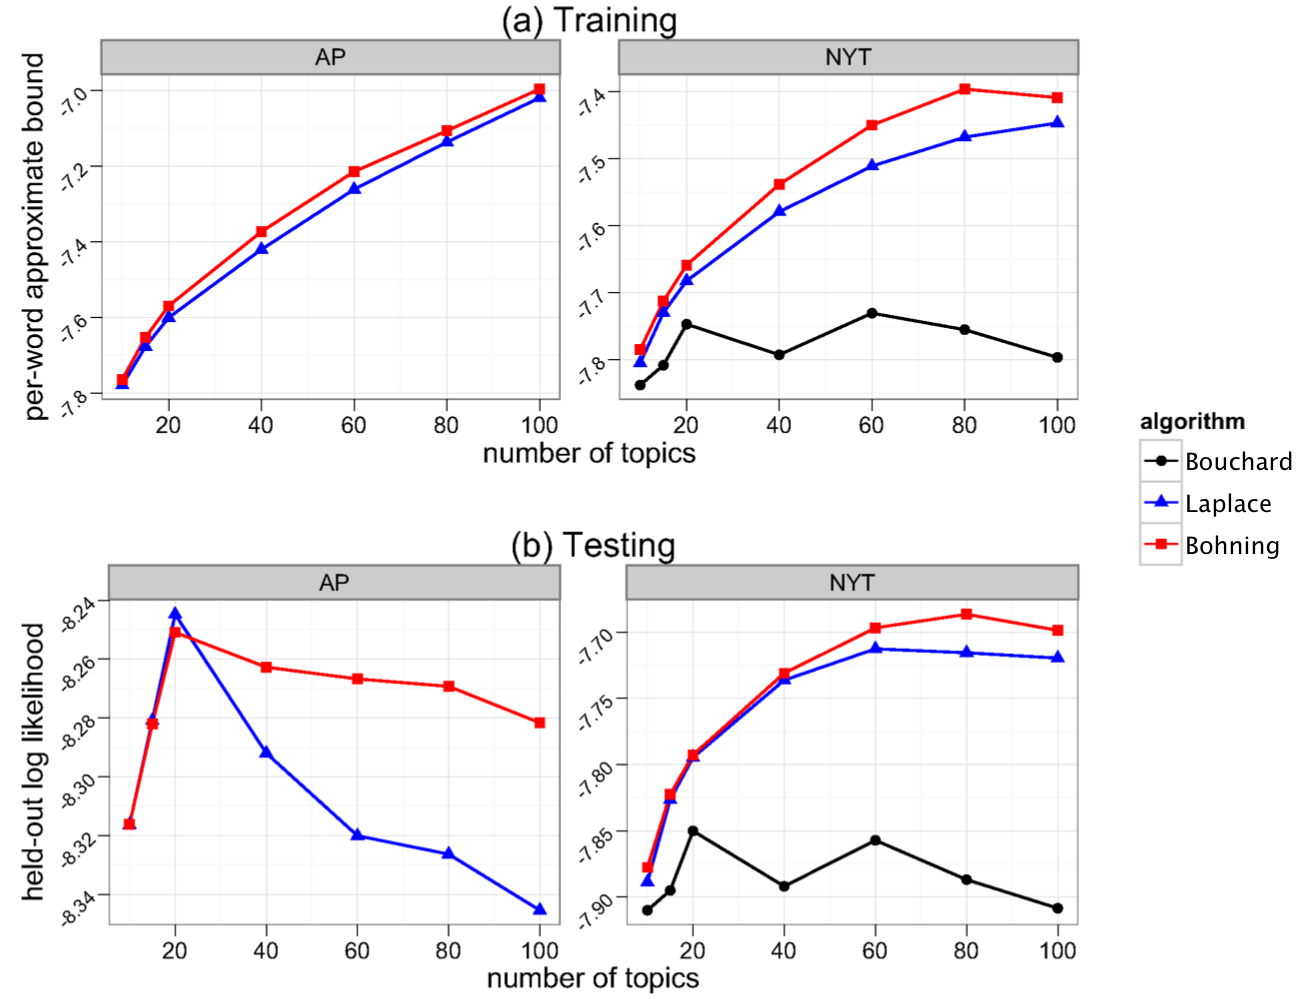
\includegraphics[height=0.40\textheight]{../Chap2/plots/figs/fig1-all-3.png}
  \caption{(a) Approximate per-word lower bound against the number of topics. A good approximation will go up as the number of topics increases, but not necessarily indicate a better predictive performance on the held out data. (b) Per-word held-out log likelihood against the number of topics. Higher numbers are better. Both nonconjugate methods perform better than Bouchard. Bohning inference performs best. Bouchard method was erratic in both collections. (It is not plotted for the AP collection.)}
  \label{fig:chap2-fig-all-3}
\end{figure}

We fit models with all three E-steps shown. To initialize nonconjugate inference we set the variational mean parameter $\mu = 0$ for log topic proportions $\theta$ and computed the corresponding updates for the topic assignments $z$. We initialize the topics in variational EM to random draws from a uniform Dirichlet.

With nonconjugate inference in the E-step, variational EM approximately optimizes a bound on the marginal probability of the observed data. We can calculate an approximation of this bound over all documents. We monitor this quantity as we run variational EM.

To test our fitted models, we measured predictive performance on held-out data with predictive distributions derived from the posterior approximations. We follow use the document-completion metric\cite{Asuncion2012} discussed in the previous chapter. We fix fitted topics and logistic normal parameters $M = 
\{\param_{1:K},\mu,\sigma\}$. We split each held-out document in to two halves $(x_d^{(e)},x_d^{(l)})$ and form the approximate posterior log topic proportions $q(\thd)$ using one of the approximate inference algorithms and the first half of the document $\xdoc$. We use this to form an approximate predictive distribution,
\begin{align}
p(\xdoc|\xdoc^{(e)}, \params) 
\approx 
\int_\thd \sum_Z p(\xdoc|z,\params)q_{\xdoc^{(e)}}(\thd) d\thd 
\approx 
\sum_k \param_k \vv{\pi}_k
\end{align}
where $\vv{\pi}_k \propto \exp(\ex{\theta_{dk}}{q}])$. Finally, we evaluate the log probability of the second half of the document using that predictive distribution; this is the held out log likelihood. A better model and inference method will give higher predictive probabilities of the unseen words. Note that this testing framework puts the approximate posterior distributions on the same playing field. The quantities are comparable regardless of how the approximate posterior is formed.

Figure \ref{fig:chap2-fig-all-3} shows the per-word approximate bound and the per-word held out likelihood as functions of the number of topics. Figure \ref{fig:chap2-fig-all-3} (a) indicates that the approximate bounds from nonconjugate inference generally go up as the number of topics increases. This is a property of a good approximation because the marginal certainly goes up as the number of parameters increases. In contrast, the Bouchard bound behaves erratically. This is illustrated for the New York Times corpus; on the Associated Press corpus, it does not come close to the approximate bound and is not plotted.

Figure \ref{fig:chap2-fig-all-3} (b) shows that on held out data, the Bouchard approach, tailored for this model, performed worse than both of our algorithms. Our conjecture is that while this method gives a strict lower bound on the marginal, it might be a loose bound and give poor predictive distributions. Our methods use an approximation which, while not a bound, might be closer to the objective and give better predictive distributions. The held out likelihood plots also show that when the number of topics increases the algorithms eventually overfit the data. Finally, note that Bohning variational inference was always better than both other algorithms.

Finally, Figure \ref{fig:chap2-fig-all-2} shows the approximate bound and the held out log likelihood as functions of running-time. From Figure \ref{fig:chap2-fig-all-2}(a), we see that even though variational EM is not formally optimizing this approximate objective, the increase at each iteration suggests that the marginal probability is also increasing. The plot also shows that Bohning inference converges faster than Laplace method inference. Figure \ref{fig:chap2-fig-all-2}  (b) confirms that Bohning inference is both faster and gives better predictive performance.



\begin{figure}
  \centering
    \hspace*{-1.5cm}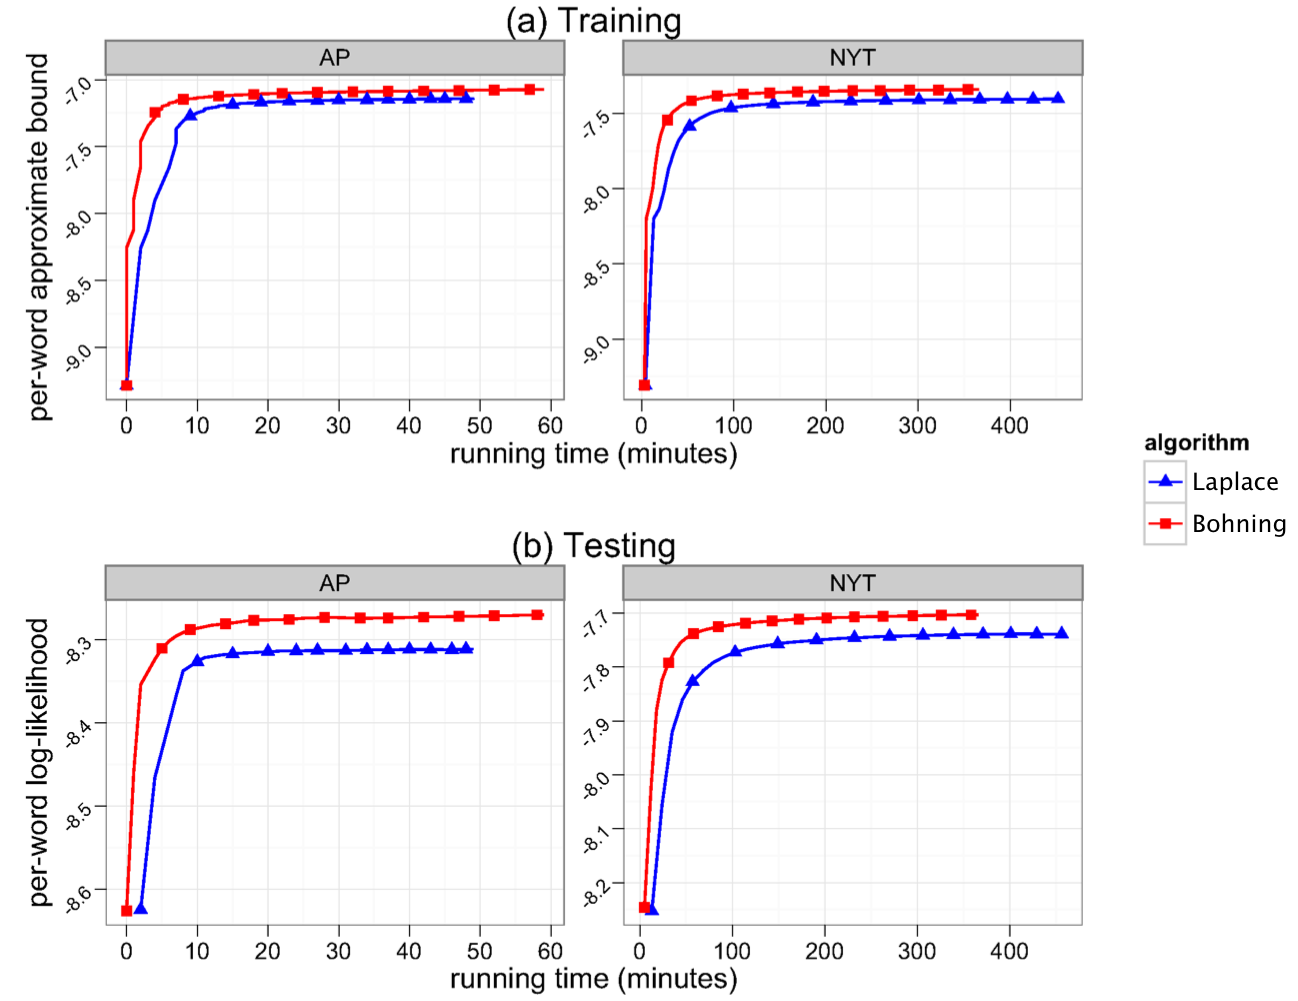
\includegraphics[height=0.40\textheight]{../Chap2/plots/figs/fig2-all-2.png}
  \caption{In this figure, we set the number of topics as K = 60. (Others are similar.) (a) The per-word approximate bound during model fitting with variational EM. Though it is an approximation of the variational EM objective, it converges in practice. (b) The per- word held out likelihood during the model fitting with variational EM. Laplace inference performs best in terms of speed and predictive performance.}
  \label{fig:chap3-fig-all-2}
\end{figure}


\section{Conclusions}
We have provided an overview of non-conjugate variational inference, with a particular emphasis on local variational approximations. We have demonstrated empirically the efficiency of local softmax bounds, and in particular the Bohning bound, which provides for rapid, guaranteed convergence.

There has of course been substantial interest in deriving inference schemes using sampling techniques. While one could derive a Metropolis-within-Gibbs sampling scheme to overcome the non-conjugacy in the model, that -- like the Laplace approximation -- involves many nested iterations and is simply too slow.

Instead, scalable sampling schemes have been derived by observing that the posterior sampling distribution $p(\thdk|\vv{\theta}_d^{\setminus k}, Z, X)$ can, through data-augmentation, be represented as a scale-mixture of Polya-Gamma distributions, allowing exact Gibb sampling. This, combined with some approximations, can be employed to create an efficient Gibb-sampling routine for inference in the CTM\cite{Chen2013}.

A more natural link-function in the case of sampling-based inference is the probit function. To our knowledge, no implementation of a correlated topic-model using the probit has been publised, likely because the probits lighter tails would make it more sensitive to outliers. Further, while deterministic inference schemes can be trivially obtained for the probit in the binary case\cite{AlbertChib1993}, in the multinomial case the inference schemes become highly complex and require the use of sampling within the variational routine to approximate certain expectations\cite{GiKa2003}.

In the remainder of this thesis we will employ the Bohning bound consistently due to its properties of speed and guaranteed convergence. In the next chapter, we will augment the correlated topic-model to employ covariates to further help assign topics to medium and short texts. 

%\subsection{Inference with the Probit}
%The probit is the CDF of a standard normal distribution:
%
%\begin{align}
%\Phi(a) = & \int_{-\infty}^{a} \phi(\epsilon) d\epsilon & \epsilon \sim \nor{0}{1}
%\end{align}
%where $\phi(\epsilon) = \frac{1}{\sqrt{2\pi}} e^{-\half \epsilon ^2}$ denotes the PDF of a standard normal. %The following identities are useful when working with the probit:
%
%%\begin{align}
%%    \Phi'(a) = & \phi(a)  & \phi'(a) = & -a \phi(a) \\
%%    1 - \Phi(a) = & \Phi(-a) & \text{ } & \text{ }
%%  \label{eqn:probit-identities}
%%\end{align}
%When working with the probit, it is useful to know that the PDF and expected value of a variable $a < X < b$ according to a truncated Gaussian distribution in the range $(a,b)$:
%\begin{align}
%X & \sim \mathcal{N}_{(a,b)}\left(\mu, \sigma \right) & \implies p(X = x) & = \frac{1}{Z} \frac{\phi (\xi)}{\sigma} \\
% & & p(X \leq x) & = \frac{1}{Z} \left( \Phi(\xi) - \Phi(\alpha)\right)
%\end{align}
%
%where $\xi = \frac{x - \mu}{\sigma}$, $\alpha = \frac{a - \mu}{\sigma}$ and $\beta = \frac{b - \mu}{\sigma}$ and the normalizing constant of the distribution is $Z = \Phi(\beta) - \Phi(\alpha)$. 
%
%Further, note that for $b = \infty$, $\Phi(\frac{b-\mu}{\sigma}) = 1$ and for $a = -\infty$, $\Phi(\frac{a-\mu}{\sigma}) = 0$ so that, for example, for a right-truncated normal distribution the normalising constant is $\Phi(\frac{b - \mu}{\sigma})$.
%
%For the fully-truncated, right-truncated, and left-truncated distributions, the expected values are defined as
%
%\begin{align}
%X & \sim \mathcal{N}_{(a,b)}\left(\mu, \sigma \right) & \implies \ex{X}{} & = \mu + \sigma \frac{\phi(\alpha) - \phi(\beta)}{Z} \label{eqn:full-trunc-mean} \\ 
%X & \sim \mathcal{N}_{(a,\infty)}\left(\mu, \sigma \right) & \implies \ex{X}{} & = \mu + \sigma \frac{\phi(\alpha)}{1 - \Phi(\alpha)} \label{eqn:left-trunc-mean} \\
%X & \sim \mathcal{N}_{(-\infty,b)}\left(\mu, \sigma \right) & \implies \ex{X}{} & = \mu - \sigma\frac{\phi(\beta)}{\Phi(\beta)} \label{eqn:right-trunc-mean}
%\end{align}
%
%
%The use of the probit is trivially motivated by a slight modification of the original logistic regression example in the introduction.
%
%Let $t_d$ be denoted by the following:
%\begin{equation}
%    t_d = \left\{ \begin{matrix}
%        1 & \text{if } y > 0 \\
%        0 & \text{if } y \leq 0
%    \end{matrix} \right.
%\end{equation}
%
%% Some presentations alternatively let $t_n \in \{-1, +1\}$ and thus be defined as $t_n = \text{sgn}(y_n)$. However this has no practical effect on the inference.
%
%Following \cite{AlbertChib1993}, define an auxiliary variable $y_n$ as
%\begin{align}
%y_d & = \vv{w}\T \vv{x}_d + \epsilon_d & \epsilon_d \sim \nor{0}{1}
%\end{align}
%which is of course the same as saying $y_d \sim \nor{\vv{w}\T\vv{x}_d}{1}$. With this, the probability that $t_d = 1$ can be written as
%\begin{equation}
%\begin{aligned}
%p(t_d = 1 | \vv{x}_d) & = p (y_d > 0) \\
%& = p(\vv{w}\T\vv{x}_d + \epsilon_d > 0) \\
%& = p(\epsilon_d > - \vv{w}\T\vv{x}_d) \\
%& = p(\epsilon_d \leq \vv{w}\T\vv{x}_d) & \text{\emph{by symmetry of the Gaussian PDF}} \\
%& = \Phi(y_d) 
%\end{aligned}
%\end{equation}
%
%A similar result can be obtained by making use of the usual identities for truncated Gaussians.
%
%\begin{equation}
%\begin{aligned}
%p(t = 1 | \vv{x}, \vv{w}) & = \int p(t = 1 | \vv{y}) p(\vv{y} | \vv{x}, \vv{w}) d\vv{y} \\
% & = \int \delta(y > 0) p(\vv{y} | \vv{x}, \vv{w}) d\vv{y} & \text{\emph{a right-truncated distribution}} \\
% & = \Phi(\vv{w}\T\vv{x}) & \text{\emph{its normalising constant}}
%\end{aligned}
%\end{equation}
%
%Compared to the logit, the probit has lighter tails, and so is more likely to be adversely affected by outliers. Additionally, the likelihood surface, for probit regression at least, is often flat near it's maximum, hindering convergence\cite{Dow2004}.
%
%The weights inferred in a probit model are harder to interpret than for the logit. The d-th weight, $w_d$ is the amount by which a Z-score is increased given the d-th covariate. Typically one uses the marginal effects:
%
%\begin{equation}
%\frac{\delta \Phi(\vv{w}\T\vv{x}_d)}{\delta x_{df}} = w_f \phi(\vv{w}\T\vv{x}_d)
%\end{equation}
%
%This metric provides the amount by which probability of the positive class is increased by every unit change in the feature $x_{df}$. Unlike the case of ordinary least squares (where the marginal effects are just $w_f$) here we need a value of $\vv{x}$ in order to evaluate the marginal effects. One approach is to use the empirical mean $\bar{\vv{x}}$: however for 1-of-F encodings of categorical features the mean will not correspond to any real-world datapoint (e.g. a person who is 49\% male and 51\% female). The alternative is the average marginal effects $\frac{w_f}{D}\sum_d\phi(\vv{w}\T\vv{x}_d)$. In practice, both approaches tend to give similar answers.
%
%
%%\fixme{See http://stats.stackexchange.com/questions/42956/how-do-i-interpret-a-probit-model-in-stata}
%
%\subsection*{Maximum Likelihood Estimation}
%With a Bernoulli distribution on $t_d$ our log-likelihood has the form
%
%\begin{align}
%\ln p(\vv{y}; X, \vv{w}) & = \sum_d t_d \ln \Phi(y_d) + (1 - t_d) \ln (1 - \Phi(y_d)) \\
%& \text{where } y_d = \vv{w}\T\vv{x}_d
%\end{align}
%
%The gradient $\vv{g}_w$ and Hessian $H_w$ of the log-likelihood with respect to $\vv{w}$ are.
%
%\begin{align}
%\vv{g}_w = & \sum_d \left( t_d \frac{\phi(y_d)}{\Phi(y_d)} - (1 - t_d) \frac{\phi(y_d)}{1 - \Phi(y_d)} \right) \vv{x}_d \label{eqn:probit-gradient}\\
%H_w = & - \sum_d \phi(y_d) \left(
%    t_n \frac{\phi(y_d) + y_d \Phi(y_d)}{\Phi(y_d)^2} + (1-t_d) \frac{\phi(y_d) + y_d (1-\Phi(y_d))}{(1 - \Phi(y_d))^2}
%\right) \vv{x}_d \vv{x}_d\T \label{eqn:probit-hessian}
%\end{align}
%
%This is sufficient to perform a Newton-Raphson update
%\begin{align}
%\vv{w}^{(\text{new})} \leftarrow \vv{w}^{(old)} - H_w^{-1} \vv{g}_w
%\end{align}
%
%although with some re-arrangement of \eqref{eqn:probit-gradient} and \eqref{eqn:probit-hessian} one can obtain an update in the form of weighted least-squares as with the logit.
%
%\begin{align}
%\vv{w}^{(new)} = \invb{X\T R X}X\T R \vv{z}
%\end{align}
%where
%\begin{align}
%R & = \diag{\left\{ \phi(y_d) \left(
%    t_n \frac{\phi(y_d) + y_n \Phi(y_d)}{\Phi(y_d)^2} + (1-t_d) \frac{\phi(y_d) + y_d (1-\Phi(y_d))}{(1 - \Phi(y_d))^2}
%\right) \right\}_{d=1}^D} \\
%z & = X \vv{w}^{(old)}  - \inv{R} \text{ vec} \left(\left\{ t_d \frac{\phi(y_d)}{\Phi(y_d)} - (1 - t_d) \frac{\phi(y_d)}{1 - \Phi(y_d)} \right\}_{d=1}^D\right)
%\end{align}
%
%
%
%\subsection*{MAP Estimation}
%Consider once again the case of logistic regression with a zero-mean Gaussian prior on the weights $\vv{w}$.
%
%\begin{align}
%\vv{w} \sim & \nor{\vv{0}}{\Lambda} & y_d | \vv{w} \sim & \nor{\vv{w}\T\vv{x}_d}{1} \\
%\text{ } & \text{ } & t_d | y_d \sim & \mathcal{B}\left( \Phi(y_d) \right)
%\end{align}
%
%Unlike the logit, estimation here is made easy by the fact that the prior is conjugate to the likelihood of the latent score $y_n$. The distribution of $y_n$ itself is conditional on $t_n$ and is made up of two disjoint, truncated Gaussians:
%
%\begin{align}
%y | t, \vv{x}, \vv{w} \sim \left\{ \begin{array}{lr} \mathcal{N}_+ (\vv{w}\T\vv{x}, 1) & t = 1 \\
%\mathcal{N}_- (\vv{w}\T\vv{x}, 1) & t = 0
% \end{array} \right.
%\end{align}
%
%Using identities for the expectation of a truncated Gaussian distribution one can obtain the following using a MAP-EM algorithm\cite{Figueiredo2003}\cite{Armagan2011}:
%
%\begin{description}
%    \item[E-Step:]  \begin{equation*}
%            \ex{y_n}{} = \left\{ \begin{matrix*}[l]
%                \wmap\T\vv{x}_d + \frac{\phi(\wmap\T\vv{x}_d)}{\Phi(\wmap\T\vv{x}_d)} & \text{if } t_d = 1 \\
%                \quad & \quad \\
%                \wmap\T\vv{x}_d - \frac{\phi(\wmap\T\vv{x}_d)}{1 - \Phi(\wmap\T\vv{x}_d)} & \text{if } t_d = 0 
%            \end{matrix*} \right.
%        \end{equation*}
%    \item[M-Step:] $\wmap \leftarrow \invb{X\T X + \Lambda^{-1}}X\ex{\vv{y}}{}$
%\end{description}
%As noted by \cite{Armagan2011} the MAP estimate is identical to the variational estimate, where the normally-distributed variational prior has covariance $\Sigma = \invb{X\T X + \Lambda^{-1}}$ and mean $\vv{\mu} = \Sigma X \ex{\vv{y}}{}$. Equally, using an improper prior (i.e. $\Lambda = 0$), the MLE and MAP estimates are identical.
%
%Making use of the posterior, it's straightforward to show that the predictive distribution is then
%
%\begin{align}
%p(t_* = 1| X, \vv{t}, x_*) & = \int_{\vv{w}} p(t_* | \vv{w})\int_{\vv{y}} p(\vv{w}| X, \vv{y})p(\vv{y}|\vv{t}) d\vv{y} d\vv{w} \\
%& = \Phi(y_*) \qquad \qquad \qquad \text{where }y_* = \vv{w}_{MAP}\T\vv{x}_*
%\end{align}
%
%%\subsection*{Gibbs Sampling}
%%Similar updates can be used for MCMC estimation techniques, where we draw $y_n$ and $t_n$ according to the following posteriors:
%%
%%\begin{align}
%%\vv{w} | \Lambda & \sim \nor{\Sigma X\T \vv{y}}{\Sigma} & \Sigma & = \left(X\T X + \Lambda^{-1}\right)^{-1} \label{eqn:sample-w}
%%\end{align}
%%\begin{align}
%%\begin{matrix}
%%y_n | t_n,x_n,\vv{w}    & \sim & \mathcal{N}_{+} \left(\vv{w}\T\vv{x}_n, 1\right) & [t_n = 1] \\
%%\quad  &  \sim & \mathcal{N}_{-} \left(\vv{w}\T\vv{x}_n, 1\right) & [t_n = 0] \\
%%\end{matrix} \label{eqn:sample-yn}
%%\end{align}
%%
%%Where we sample $y_n$ from a truncated normal distribution.
%
%%\subsection{Bayesian Probit Regression with Gaussian Processes}
%%As with the Logit
%
%
%\subsection*{Extending the Probit to the Multinomial Case}
%In case of the multinomial probit case, as with the multinomial logit, one learns $L$ independent weight vectors $\vv{w}_l$ from which we define the auxiliary variable $\vv{y} \sim \nor{W\vv{x}}{1}$ where $W = \{ \vv{w}_l\T \}_{l=1}^L$. The prediction rule also necessarily changes, becoming:
%
%\begin{align}
%t_{dl} = \left\{ \begin{array}{lr} 1 & \text{if } y_{dl} > y_{dj} \quad \forall j \neq l \\ 0 & \text{otherwise} \end{array} \right.
%\end{align}
%
%In the binary model, the conditional distribution on the scalar $y$ given $t$ involves decomposing the $\mathbb{R}$ space into $\mathbb{R}_-$ and $\mathbb{R}_+$, with corresponding disjoint, truncated Gaussian distributions. In the multinomial model, the conditional distribution of the vector $\vv{y} \in \VReal{L}$ involves decomposing the $\VReal{L}$ space into $L$ cones $C_l = \{ \vv{y} : y_l > y_j \forall l \neq j \}$, each of dimension L, such that $\bigcup_l C_l = \VReal{L}$. The conically truncated Gaussian distribution for a label $l$ is denoted as $y_n \sim \mathcal{N}^{l}\left(W\vv{x}, 1\right)$. 
%
%From \cite{Girolami2007} we see that predictive distribution is:
%\begin{equation}
%\begin{aligned}
%p(t_{dl} = 1 | \vv{x}, \{ \vv{w}_j\T \}_{j=1}^L) & =
%\int \delta (y_{dl} > y_{dk} \forall k \neq l) \prod_j p(y_{dj} | \vv{w}_j\T\vv{x}) d\vv{y} \\
%&= \int_{C_l} \prod_j p(y_{dj} | \vv{w}_j\T\vv{x}) d\vv{y} \\
%&= \ex{\prod_{j \neq l} \Phi(\epsilon + m_{dl} - m_{dj})}{p(\epsilon)}
%\end{aligned}
%\end{equation}
%where $\epsilon \sim \nor{0}{1}$ and $m_{dl} \sim \nor{\vv{w}_l\T\vv{x}_d}{\sigma^2}$. Further, also from \cite{Girolami2007}, we obtain the posterior expectation over $y_{dl}$ for $t_{dl} = 1$
%\begin{align}
%\ex{\vv{w}_l\T\vv{x}_d}{q} + \sum_{k \neq l} \left(\ex{\vv{w}_k\T\vv{x}_d}{q} - \ex{y_{dk}}{q}\right)
%\end{align}
%and for $y_{nk}$ for all $t_{dk} = 0$
%\begin{align}
%\begin{split}
%\ex{\vv{w}_k\T\vv{x}_d}{q}
% - Z_d^{-1}\mathbb{E}_{p(\epsilon)} [ & \phi\left(\ex{\vv{w}_k\T\vv{x}_d}{q} - \ex{\vv{w}_l\T\vv{x}_d}{q} \right) \\
% & \prod_{j \neq l,k}\Phi\left(\epsilon + \ex{\vv{w}_l\T\vv{x}_d}{q} - \ex{\vv{w}_i\T\vv{x}_d}{q} \right) ]
%\end{split}
%\end{align}
%where $Z_d = p(\vv{y}_d \in \mathcal{C}) = \ex{\prod_{j \neq l}\Phi\left(\epsilon + \ex{\vv{w}_l\T\vv{x}_d}{q} - \ex{\vv{w}_i\T\vv{x}_d}{q} \right) }{p(\epsilon)}$. Given these expectations, closed form updates for the weights can be obtained, however the expectation $\ex{y_dk}{q}$ can only be evaluated using quadrature or sampling methods.
%
%
%\section{Other Inference methods}
%\begin{enumerate}
%    \item Sampling, reference the large-scale paper
%    \item Discussion of the probit, reference Mark's paper.
%\end{enumerate}
%

%\chapter{Comparison between the Logit and the Probit}
%In the following we implement a correlated topic model\cite{Blei2006} using the Bohning-bounded logit and the probit. As the normal distribution has much lighter tails than the logistic distribution (of the order of $\exp(y^2)$ instead of $\exp(y)$), it is much less accommodating of outliers. We would therefore expect slower convergence in the early iterations as we attempt to fit the noise.

\bibliographystyle{plain}
\bibliography{/Users/bryanfeeney/Documents/library.bib}

\end{document}

